% !TEX root = ../thesis.tex

\chapter{Extending BibLaTeX and JabRef with Entry Type for Standards}

Standards, e.g.\ ISO or DIN standards, are a document type that is not very well supported by the standard BibLaTeX entry types. However, Katharina Großer provided a BibLaTeX driver\footnote{cf.\ document class file \texttt{rgseThesis.cls}} to deal with the special fields and format that often describe standards.

JabRef\footnote{\url{https://www.jabref.org}} can be used to manage your bibliography. It can easily be extended to handle the entry type \texttt{standard}. Use the menu \emph{BibTeX -- Customize Entry Type} to add the new type. See \prettyref{fig:jabref} for details.

\begin{figure}
    \centering
    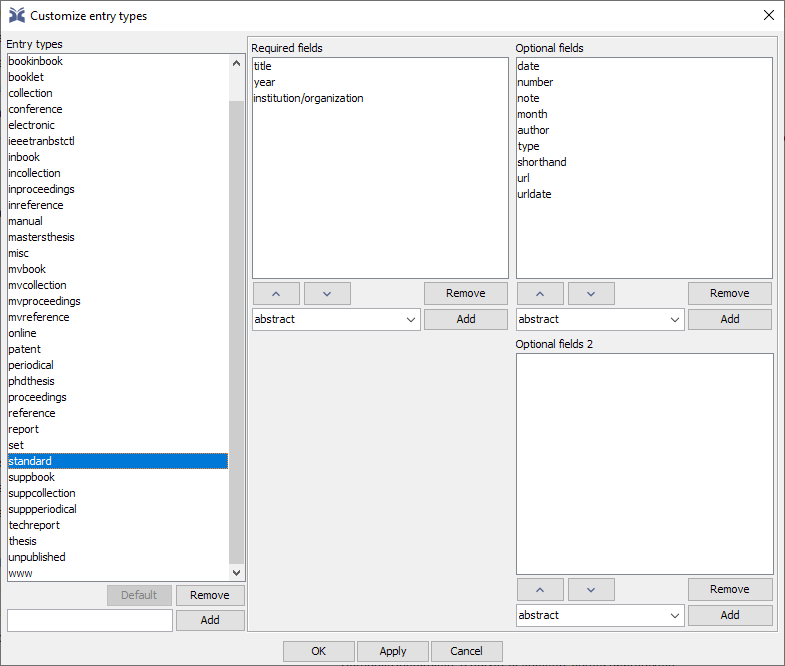
\includegraphics[height=10cm]{images/JabRef}
    \caption{Settings for entry type \texttt{standard}\label{fig:jabref}}
\end{figure}

Here are some cites to test for the bibliography entry type \texttt{standard}: ISO 25964 \cite{ISO20111TI, ISO20132IO} defines an international standard for glossaries.

\cleardoublepage
